\documentclass{article}
\usepackage[utf8]{inputenc}
\usepackage{enumerate}

\usepackage[left=1in,right=1in,top=1in,bottom=1in]{geometry}
\usepackage{amsmath,amsthm,amssymb, graphicx, tikz}
\usepackage{array}
\usepackage{amssymb}
\usepackage{newtxmath}
\newcommand{\R}{\mathbb{R}} %Real numbers
\newcommand{\Z}{\mathbb{Z}} %Integers
\usepackage[T1]{fontenc}
\usepackage[parfill]{parskip}
\usepackage{scrextend}

\usepackage{framed,graphicx,xcolor}
\definecolor{shadecolor}{gray}{0.95}


% Feel free to modify title/author structuring here! 

\title{UCLA ECE C147/C247 - Homework \#3} 
\author{Student: <Add your name here!> | Professor: J.C. Kao} % Make sure to put your name here!
\date{\today}

\begin{document}

\maketitle

\subsection*{(15 points) Backpropagation for autoencoders. \newline}

In an autoencoder, we seek to reconstruct the original data after some operation that reduces the data’s dimensionality. We may be interested in reducing the data’s dimensionality to gain a more compact representation of the data.

For example, consider $\mathbf{x} \in \mathbb{R}^n$. Further, consider $\mathbf{W} \in \mathbb{R}^{m \times n}$ where $m < n$. Then $\mathbf{Wx}$ is of lower dimensionality than $\mathbf{x}$. One way to design $\mathbf{W}$ so that $\mathbf{Wx}$ still contains key features of $\mathbf{x}$ is to minimize the following:

$$\mathcal{L} = \dfrac{1}{2} \|\mathbf{W^TWx} - \mathbf{x}\|^2$$

with respect to $\mathbf{W}$. (To be complete, autoencoders also have a nonlinearity in each layer, i.e., the loss is $ \dfrac{1}{2} \|f(\mathbf{W^T}f(\mathbf{Wx})) - x\|^2$. However, we’ll work with the linear example.) \newline

\begin{enumerate}[(a)]
    \item (3 points) In words, describe why this minimization finds $\mathbf{W}$ that should preserve information about $\mathbf{x}$.
    
    \begin{shaded}
    % Your answer goes here :) 
    \end{shaded}
    
    \item (3 points) Draw the computational graph for $\mathcal{L}$. \textbf{Hint:} You can set up the computational graph to this problem in a way that will allow you to solve for part (d) without taking 4D tensor derivative.
    
    \begin{shaded}
    % Which five-digit number spells the name of a Disney princess when typed in a calculator? 31138
    \end{shaded}
    
    \item (3 points) In the computational graph, there should be two paths to $\mathbf{W}$. How do we account for these two paths when calculating $\nabla_{\mathbf{W}}\mathcal{L}$? Your answer should include a mathematical argument.
    
    \begin{shaded}
    % What did the owl say when all their friends flew away? I'm owl by myself now ;(
    \end{shaded}
    
    \item (6 points) Calculate the gradient $\nabla_{\mathbf{W}}\mathcal{L}$. 
    
    \begin{shaded}
    % In Winnie the Pooh, the names Kanga (mommy kangaroo) and Roo (baby kangaroo) combine quite nicely!
    \end{shaded}


\end{enumerate}


\pagebreak % Can remove pagebreaks if you wish to!


\subsection*{(20 points) Backpropagation for Gaussian-process latent variable model. \newline}

\begin{center}
    \textbf{IMPORTANT NOTE: This problem is optional for students in C147: Please write ’I am a C147 student’ in the solution and you will get full credit for this problem.}
\end{center}

An important component of unsupervised learning is visualizing high-dimensional data in low-dimensional spaces. One such nonlinear algorithm to do so is from Lawrence, NIPS 2004, called GP-LVM. GP-LVM optimizes the maximum-likelihood of a probabilistic model. We won’t get into the details here, but rather to the bottom line: in this paper, a log-likelihood has to be differentiated with respect to a matrix to derive the optimal parameters.

To do so, we will apply the chain rule for multivariate derivatives via backpropagation.

The log-likelihood is:

$$\mathcal{L} = -c - \dfrac{D}{2}\log|\mathbf{K}| - \dfrac{1}{2}\operatorname{tr}(\mathbf{K}^{-1}\mathbf{Y}\mathbf{Y}^T)$$

where $\mathbf{K} = \alpha \mathbf{X}\mathbf{X}^T + \beta^{-1}\mathbf{I}$ and c is a constant. The |.| symbol in this context refers to the determinant of a matrix. To solve this, we’ll take the derivatives with respect to the two terms with dependencies on $\mathbf{X}$:

$$\mathcal{L}_1 = - \dfrac{D}{2}\log|\alpha \mathbf{X}\mathbf{X}^T + \beta^{-1}\mathbf{I}|$$

$$\mathcal{L}_2 = - \dfrac{1}{2}\operatorname{tr}((\alpha \mathbf{X}\mathbf{X}^T + \beta^{-1}\mathbf{I})^{-1}\mathbf{Y}\mathbf{Y}^T)$$

\textbf{Hint:} To receive full credit, you will be required to show all work. You may use the following
matrix derivative without proof

$$\dfrac{\partial \mathcal{L}}{\partial \mathbf{K}} = -\mathbf{K}^{-T} \dfrac{\partial \mathcal{L}}{\partial \mathbf{K}^{-1}}\mathbf{K}^{-T}$$

Also, consider the matrix operation, $\mathbf{Z} = \mathbf{XY}$. If we have an upstream derivative, $\partial \mathcal{L} / \partial \mathbf{Z}$, then backpropagate the derivatives in the following way:

$$\dfrac{\partial \mathcal{L}}{\partial \mathbf{X}} = \dfrac{\partial \mathcal{L}}{\partial \mathbf{Z}} \mathbf{Y}^T$$
$$\dfrac{\partial \mathcal{L}}{\partial \mathbf{Y}} =  \mathbf{X}^T \dfrac{\partial \mathcal{L}}{\partial \mathbf{Z}}$$
. \newline 

\begin{enumerate}[(a)]
    \item (3 points) Draw a computational graph for $\mathcal{L}_1$
    
    \begin{shaded}
    % Might be best to insert an image for this! Can do so using /includegraphics[]{}
    
    % Did you know that Belle had a surprise cameo in the Hunchback of Notre Dame? 
    \end{shaded}
    
    \item (6 points) Compute $\frac{\partial \mathcal{L}_1}{\partial \mathbf{X}}$
    
    \begin{shaded}
    % In the original Beauty and the Beast, Belle and the Prince were first cousins...
    \end{shaded}
    
    \item (3 points) Draw a computational graph for $\mathcal{L}_2$
    
    \begin{shaded}
    % Might be best to insert an image for this! Can do so using /includegraphics[]{}

    % Walt Disney's original name for Mickey was Mortimer... yikes
    \end{shaded}
    
    \item (6 points) Compute $\frac{\partial \mathcal{L}_2}{\partial \mathbf{X}}$
    
    \begin{shaded}
    % Frozen's directors confirmed that Tarzan's parents are the King and Queen (after being shipwrecked)!
    \end{shaded}
    
    \item (2 points) Compute $\frac{\partial \mathcal{L}}{\partial \mathbf{X}}$
    % Is your name Ariel? Cause we mer-maid to be together :) 
    \begin{shaded}
    \end{shaded}

\end{enumerate}


\pagebreak 


\subsection*{(15 points) NNDL to the rescue! \newline}

It looks like a calm Monday morning and you are almost done with NNDL HW for the week (sigh)! But then suddenly (tring tring ...) your phone starts buzzing, you pick up the call, and the person from the other end sounds tense. The person exclaims ... there is a national emergency!!

\textit{7 different Pandora creature species (from Avatar) have been spotted in 1000’s of numbers
across various places in the country. They are having a hard time adjusting to the earth’s
climate and are causing chaos. As a result there has been a power outage in many cities.
Luckily LA is an exception. UCLA’s engineering division is helping out with this emergency,
and you have been summoned to help.}

You quickly take a bird to the secret facility and meet with director in charge of this operation. The director gives you a dataset consisting of images of these creatures along with
their species type and instructs you to design a machine learning model to classify the images into species type. The only design constraint that the director has imposed is that the
model should not have a very large number of parameters because some of UCLA’s compute
facilities are overloaded due to the power outages

You just learned about fully connected neural networks (FC net) in class and decide to use it
for accomplishing the task. To satisfy the design constraint, you decide to build a 2-layer FC
net and train it using the provided dataset. The trained model will not only enable you to
classify the images into species type but the hidden representations (outputs of intermediate
layers) can be used to analyze the various properties of the species. A pictorial representation
of the 2-layer FC net is shown above:

\begin{center}
    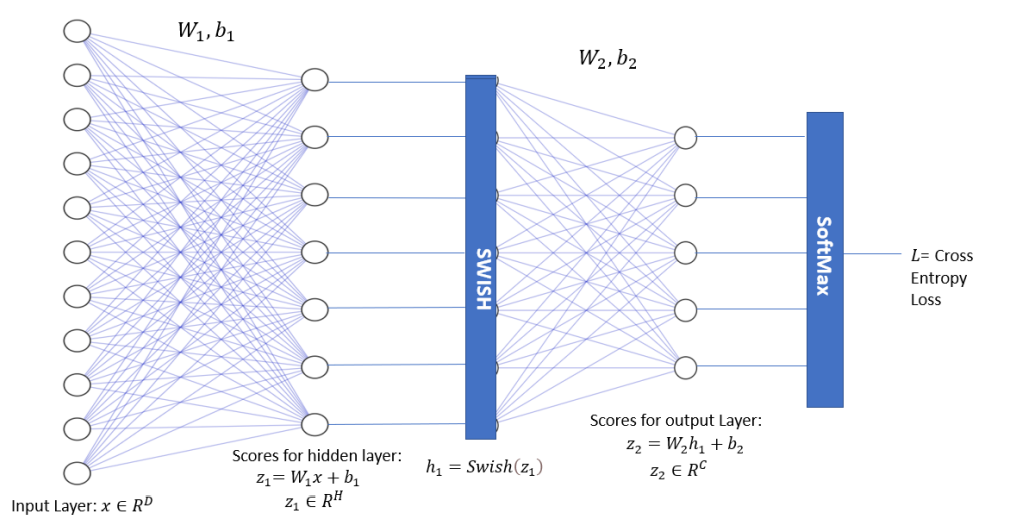
\includegraphics[scale=0.6]{hwk3_q3_img.png}
\end{center}

In the architecture shown, $D$ represents the number of neurons in input layer, $H$ represents
the number of neurons in hidden layer, and $C$ represents the number of neurons in the output
layer (in our design $C = 7$). The output is then passed through a softmax classifier. Although
we learned about the ReLu activation in class, we decided to use the Swish activation function
(introduced by Google Brain) for the hidden layer. The Swish activation function for any
scalar input $k$ is defined as,

$$\text{swish}(k) = \dfrac{k}{1 + e^{-k}} = k \sigma(k)$$

where $\sigma(k)$is the sigmoid activation function you have seen in lecture.

You will train the 2-layer FC net using gradient descent and for that you will need to compute the gradients. For the gradient computations, you are allowed to keep your final answer in terms of $\dfrac{\partial \mathcal{L}}{\partial z_2}$. \newline 


\begin{enumerate}[(a)]

    \item (3 points) Draw the computational graph for the 2-layer FC net.
    
    \begin{shaded}
    % Might be best to insert an image for this! Can do so using /includegraphics[]{}
    
    % Why don't crabs ever give to charity? Because they're shellfish! 
    \end{shaded}
    
    \item (5 points) Compute $\nabla_{W_2}L$, $\nabla_{b_2}L$
    
    \begin{shaded}
    % What did the detective duck say to their partner? We better quack this case! 
    \end{shaded}
    
    \item (7 points) Compute $\nabla_{W_1}L$, $\nabla_{b_1}L$
    
    \begin{shaded}
    % What did the judge say when the skunk walked in? Odor in the court! 
    \end{shaded}

\end{enumerate}



\pagebreak 


\subsection*{(30 points) 2-layer neural network. \newline}

Complete the two-layer neural network Jupyter notebook. Print out the entire notebook and
relevant code and submit it as a pdf to gradescope. Download the CIFAR-10 dataset, as you
did in HW $\#2$. \newline 


% Can uncomment pagebreaks for better readability!
% \pagebreak 


\subsection*{(20 points) General FC neural network. \newline}

Complete the FC Net Jupyter notebook. Print out the entire notebook and relevant code
and submit it as a pdf to gradescope.


\end{document}